\documentclass[11pt,a4paper,openany,oneside,parskip=half*]{article}

\usepackage[utf8]{inputenc}
\usepackage{tocloft}
\usepackage{nomencl}
\usepackage{pdfpages}
\usepackage{scrextend}
\usepackage{bm}
\usepackage{cite}
\usepackage{amsmath}
\usepackage{graphicx}
\usepackage[justification=justified]{caption}
\usepackage{float}
\usepackage{multicol}
\usepackage{float}
\usepackage[section]{placeins}
\usepackage[english]{babel} 
\usepackage{geometry} %Gr�ߟe des Bodys innerhalb der Seite 
\usepackage[utf8]{inputenc} 
\usepackage{ifthen}
\usepackage{caption}

%bindet die benutzten Packages ein

\linespread{1.25}

\captionsetup{width=0.485\linewidth}

\RequirePackage{ifthen}
\renewcommand{\nomgroup}[1]{%
  \ifthenelse{\equal{#1}{R}}{\item[\textbf{Roman Symbols}]}{%
    \ifthenelse{\equal{#1}{G}}{\item[\textbf{Greek Symbols}]}{%
      \ifthenelse{\equal{#1}{O}}{\item[\textbf{Operators}]}{%
	\ifthenelse{\equal{#1}{A}}{\item[\textbf{Acronyms}]}{}}}}}%
	
\renewcommand*\vec[1]{\boldsymbol{#1}}
\renewcommand*\matrix[1]{\boldsymbol{#1}}

\captionsetup[figure]{font=footnotesize}

\cftsetindents{section}{0em}{2.65em}   
\cftsetindents{subsection}{1.5em}{3em}   
\cftsetindents{subsubsection}{2.5em}{3.5em}
%setzt die fettgedruckte Schreibweise fuer Vektoren und Matrizen

\geometry{top=3cm, bottom=4cm}
\geometry{bindingoffset=1.5cm} %offset zum binden
\newcommand{\HRule}{\rule{\linewidth}{0.5mm}}  % definere gerade Linie mit 0.5mm Dicke

\makeindex %

\begin{document}
\begin{titlepage}
\begin{figure}[htp]
\vspace*{-3cm} 
\hspace*{2.7cm}  

\includegraphics{./Titelseite/rwth_aia_en_rgb.eps}
\end{figure}
\begin{center}
\textbf{Diese Arbeit wurde vorgelegt am Aerodynamischen Institut}
\end{center}
\begin{center} % ab hier zentriert
\vspace*{4.2cm} %lasse 4.5 cm Platz von oben
{ \huge \bfseries Investigations on two-way coupling effects of particle-laden decaying isotropic turbulent flows}\\[0.3cm] % Groߟe Buchstaben, fett gedruckt, lasse 0.3cm Platz nach unten
\HRule \\[0.5cm] %Linie, 0,5cm Platz nach unten
\textsc{\Large{Projektarbeit}}\\ %in Kapitälchen
\textsc{\Large{von}}\\
\textsc{\LARGE{Julian Stemmermann, Steffen Trienekens und Christian Soika}}\\[0.5cm]
\HRule \\[0.4cm]
{\Large{Aerodynamisches Institut der RWTH Aachen}}\\[.5cm]
{\large \today} \\[1.5cm] % heutiges Datum
\vfill % So viel Platz lassen, dass es bis zur Ende der Seite geht, wobei die Abstände bei dem nächsten vfill gleich sind
\begin{flushleft} \large  %Einrückung, groß
\begin{tabular}{ll} % Tabelle
Betreuer: &Konstantin Fr\"ohlich \\
Erstpr\"ufer: &Univ.-Prof.\,Dr.-Ing. Wolfgang Schr\"oder
\end{tabular}
\end{flushleft}
\vfill % So viel Platz lassen, dass es bis zur Ende der Seite geht
\end{center}
\end{titlepage}

\numberwithin{equation}{section} %bestimmt die Nummerierung der Gleichungen, in diesem Fall nach Kapitel anstatt sie einfach durchzunummerieren

\makenomenclature %erstellt und druckt die Nomenklatur-Tabelle


\renewcommand{\refname}{}
\renewcommand{\nomname}{}



\setlength{\columnsep}{30pt}
\setlength{\parindent}{0pt}

\pagebreak
\tableofcontents{} %erstellt die Inhaltsangabe
\thispagestyle{empty}
\pagebreak

\renewcommand{\thesection}{\Roman{section}}
\pagenumbering{Roman} 

\section{Nomenclature}
\printnomenclature
\pagebreak
\renewcommand{\thesection}{\arabic{section}}
\setcounter{section}{0}
\section{Introduction}
\pagenumbering{arabic}
\setcounter{page}{1}
\begin{figure}[h]
	\centering
  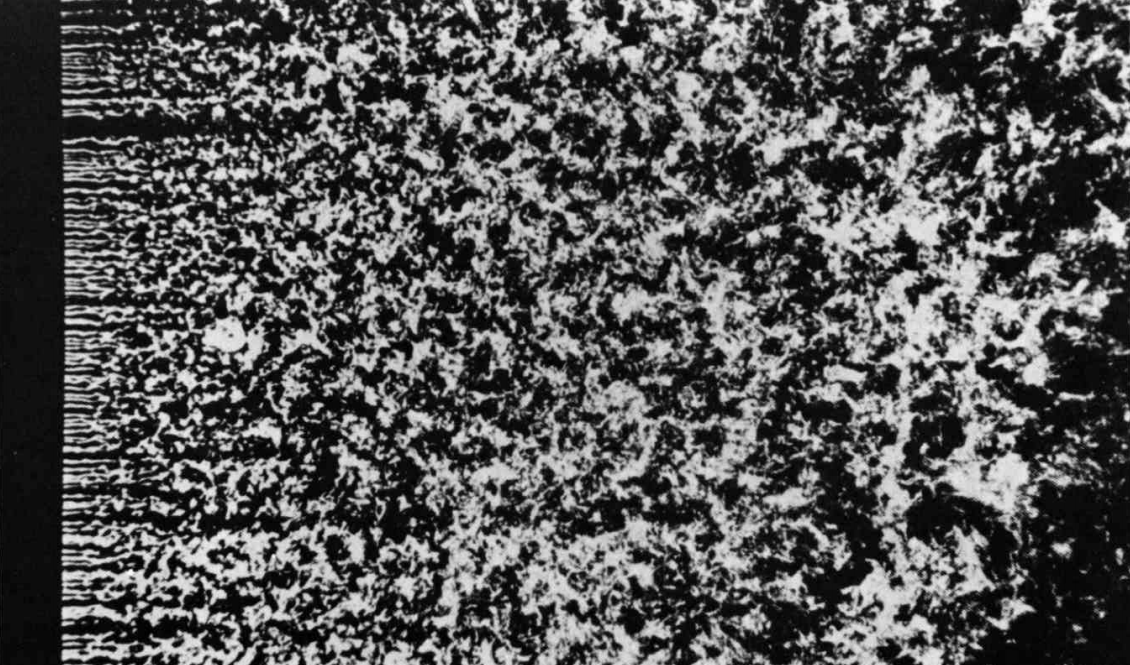
\includegraphics[width=\textwidth]{./Abbildungen/TurbulentMotion_Introduction.png}
  \captionsetup{width=0.97\linewidth}
	\caption{Photograph courtesy of Hassan Nagib and Thomas Corke: Formation of an nearly isotropic turbulent flow field behind a grid. Source: \cite{albumOfTurbulentMotion}}
	\label{introduction_picture}
\end{figure}
<<<<<<< HEAD
This work deals with the effects of particles on the flow conditions of isotropic turbulent flows.
There are many examples of these particle-laden turbulent flows in nature, e.g. in volcanic eruptions and in the "white water" of breaking waves.
\newline
Multiphase flows also occur in many technical applications. Spray automization in fuel injectors, cyclonic particle separation in oil refineries and sediment accumulation in pipelines are just three of many cases, where it is of huge interest to predict the influence of particles on the turbulence of the flow.
Of major industrial interest are the fuel dispersion and combustion in an petrol-powered engine. To get a homogeneous and fast combustion, both should take place at turbulent flow conditions. One could say it is an important question, in which way and intensity the particles influence the turbulence.
=======
Particle laden turbulent flows are ubiquitous in nature, e.g. in volcanic eruptions and in the "white water" of breaking waves.
Spray automization in fuel injectors, cyclonic particle separation in oil refineries and sediment accumulation in pipelines are examples of technical applications, where it is of huge interest to predict the impact of particles on turbulent flows.
Turbulence augmentation or attenuation by particles is therefore a decisive factor.
>>>>>>> 4113d64895656e6ba27b195eb1861d9a73879796
\newline
A study on the impact of particles on the flow conditions of isotropic turbulent flows is presented at hand.
In this work the influence of the particles on the conditions is presented. Analyzing the energy transfer between particles and fluid will be focused.  
\newline
<<<<<<< HEAD
In this work the influence of the particles on the streaming conditions is presented by using DNS and LES simulations. The focus lies on analyzing the energy transfer between particles and fluid as well as the intensity of the decrease of turbulent kinetic energy in the fluid.  
At the beginning some mathematical background information about modeling turbulent single phase and particle-laden flows are given. 
Additionally the Navier-Stokes equations and the different scales of turbulent motion are presented as an approach to modelling turbulence. For particle-laden flows the equations of motion are expanded by a new term that describes the forces acting between fluid and particles. 
Also the coupling rate that describes the exchanged energy and the computational basics of methods used in this work are introduced. 
According to the computational basics the simulation methods DNS and LES, how they work and in which case which one is used is explained.
Then the used discretization method to integrate the particle tracking equations, which is a predictor-corrector-scheme, is described.     
Finally the computational method 'particle clustering' is introduced. This approach aims to decrease the computational effort of particle-laden simulations. It works the following way: the particles are coupled to clusters and each cluster is considered as one particle.
\newline
In the following the deviations caused by using this method are determined and the applicability is evaluated. Therefore the influence of the number of particles per cluster on the accuracy of the plots of the turbulent kinetic energy and the exchanged energy between particles and fluid per time is identified.
=======
First, some mathematical background information about modeling single phase and particle laden flows are given. 
Additionally, the scales of turbulent motion are described.
According to the computational basics the simulation methods DNS and LES, how they work and in which case which one is used is explained.
Then the used discretization method to integrate the particle tracking equations is described.     
Finally the computational method 'particle clustering' is introduced. 
In the following the deviations caused by using this method are determined and the applicability is evaluated.
>>>>>>> 4113d64895656e6ba27b195eb1861d9a73879796
Also the number of particles that is needed to get consistent average values for the flow characteristics is investigated.

-Due to the small particle concentration, a popular method to describe these flows is the point-particle approach, which means that every particle is treated as a mathematical point source of mass, momentum and energy.
\nomenclature[aDNS]{DNS}{Direct numerical simulation}
\nomenclature[aLES]{LES}{Large eddy simulation}
\nomenclature[aSGS]{SGS}{Subgrid scale}
\nomenclature[asP]{sP}{Single-phase simulation}
\nomenclature[aPP]{PP}{Particle-laden simulation}
\nomenclature[aILES]{ILES}{Implicit large-eddy simulation}
\pagebreak
\section{Mathematical models}%Einleitung unbedingt noch bearbeiten! 2017-10-16
\subsection{Single phase flow} %Christian
In this section, the mathematical models are introduced, which describe turbulent flows. For a more detailed description, see e.g. \cite{turbulentFlows}.
\newline%"Here should be a description what will follow, and the general structure of the chapter."
\subsubsection{Equations governing the fluid phase}
The conservation of mass, momentum and energy for a control volume reads
\nomenclature[oN]{$\vec\nabla$}{Nabla operator} %Erstellt automatisch die Nomenclature-Liste
\nomenclature[rQ]{$\vec{Q}$}{Vector of conservative Eulerian variables}
\nomenclature[rH]{$\vec{\bar{H}}$}{Flux tensor}
\begin{equation}
  \int\limits_V \frac{\partial{\vec{Q}}}{\partial{t}} \, \mathrm{d} V+ \int\limits_{\partial{V}} \vec{\bar{H}} \cdot \vec{n} \, \mathrm{d} A = \vec0.
\end{equation}
with time $t$ and the flux tensor $ \vec{\bar{H}} $.
The vector $ \vec{Q} $ contains the variables fluid density $ \rho $, 
fluid velocity $ \vec{u} $ and specific inner energy $ E $: 
\nomenclature[gr]{$\rho$}{Fluid density}
\nomenclature[ru]{$\vec{u}$}{Fluid velocity}
\nomenclature[rE]{$E$}{Specific inner energy}
\begin{equation}
 \vec{Q}= \left( \begin{array}{c}\rho\\\rho \vec{u}\\\rho E \end{array} \right).
\end{equation}
$\vec{\bar{H}} $ is the flux tensor which contains the inviscid and viscous flux, i.e.:
\nomenclature[rHi]{$\vec{\bar{H}^\mathrm{i}}$}{Inviscid part of the flux tensor}
\nomenclature[rHv]{$\vec{\bar{H}^\mathrm{v}}$}{Viscous part of the flux tensor}
\nomenclature[rp]{$p$}{Pressure}
\nomenclature[rRe]{$Re$}{Reynolds number}
\nomenclature[gt]{$\matrix{\bar{\tau}}$}{Stress tensor}
\nomenclature[rq]{$\vec{q}$}{Heat conduction vector}
\begin{equation}
\vec{\bar{H}} = \vec{\bar{H}^\mathrm{i}} + \vec{\bar{H}^\mathrm{v}} = 
 \left( \begin{array}{c}\rho \vec{u}\\\rho \vec{u} \vec{u} + p\\\vec{u} (\rho E + p) \end{array} \right) - 
 \frac{1}{Re} \left( \begin{array}{c}\ 0 \\ \matrix{\bar{\tau}}\\ \matrix{\bar{\tau}} \vec{u} + \vec{q} \end{array} \right)
\end{equation} %hier weiter Julian 2017-10-16
$ \vec{\bar{H}^\mathrm{i}} $ contains the variables that are independent of the fluid's viscosity and $ \vec{\bar{H}^\mathrm{v}} $ represents the effects of viscosity $\matrix{\bar{\tau}}$ and heat conduction $\vec{q}$. The Reynolds number 
$ Re = \frac{\rho v d}{\mu} $ is defined to be the ratio of inertia forces to viscous forces. This is also due to the 
fact that two familiar objects with Re being identical behave similar in flows.
To solve the Navier-Stokes equations, more information regarding some variables is required. For calculating the specific inner energy $ E $ 
and the heat conduction $ \vec{q} $, the following equations are used
\nomenclature[gg]{$\gamma$}{Isentropic exponent}
\nomenclature[re]{$e$}{Specific internal energy}
\nomenclature[rPr]{$Pr$}{Prandtl number}
\nomenclature[gm]{$\mu$}{Dynamic viscosity}
\begin{equation}
 E = e  \frac{1}{2} \vec{|u|}^2,
\end{equation}
\begin{equation}
 \vec{q} = - \frac{\mu}{Pr (\gamma - 1)} \vec\nabla T,
\end{equation}
with 
\nomenclature[rcp]{$c_\mathrm{p}$}{Specific isobaric heat capacity}
\nomenclature[rcv]{$c_\mathrm{v}$}{Specific isochoric heat capacity}
\begin{equation}
 \gamma = \frac{c_p}{c_v}
\end{equation}
and the Prandtl number
\nomenclature[rkt]{$k_\mathrm{t}$}{Thermal conductivity}
$ Pr = \frac{\mu_\infty c_\mathrm{p}}{k_\mathrm{t}}$
using the specific heat capacities of the fluid $ c_\mathrm{v} $ and $ c_\mathrm{p} $.
Assuming that the fluid is a newtonian fluid, the linear correlation between stress and the rate of strain results in:
\nomenclature[rI]{$\matrix{\bar{I}}$}{Identity tensor}
\nomenclature[rS]{$\matrix{S}$}{Rate-of-strain tensor}
\nomenclature[rT]{$T$}{Temperature}
\begin{equation}
 \matrix{\bar{\tau}} = 2 \mu \matrix{\bar{S}} - \frac{2}{3} \mu (\vec\nabla \cdot \vec{u}) \matrix{\bar{I}},
\end{equation}
in which $ \matrix{\bar{S}} = \frac{(\vec\nabla \vec{u})(\vec\nabla \vec{u})^T}{2} $ denotes the rate-of-strain tensor. Additionally, the viscosity
$ \mu $ can be approximated by Sutherland's law, which is based on the ideal gas-theory
\nomenclature[rS]{$S$}{Sutherland temperature}
\nomenclature[rR]{$R$}{Specific gas constant}
\begin{equation}
 \mu (T) = \mu_\infty \biggl(\frac{T}{t_\infty}\biggl)^{3/2} \frac{T_\infty + S}{T + S},
\end{equation}
where S is the Sutherland temperature.
To achieve closure the caloric state equation $ e = c_\mathrm{v} T $ and the state equation for an ideal gas $
p = \rho R T $ are used. The specific gas constant is determined by $ R = c_\mathrm{p} - c_\mathrm{v} $. 
\pagebreak
\subsection{Scales of turbulent flows}
Turbulent flows contain eddies, which are induced by reverse currents in the flow, of all sizes and shapes. Large-scale eddies bring energy to the flow which is then passed down to smaller-scales, and finally dissipated into heat by viscous effects. This behavior is called the 'energy cascade' and was first described by Richardson in the year 1920 \cite{Richardson1920}. The theory then was further developed by Kolmogorov \cite{Kolmogorov1941}. The main difference is that Kolmogorov added hypothesises like the statistical isotropy of small-scale turbulent motions and the decrease of the velocity and timescales with the decrease of the length scale along the energy cascade.
\newline
The first set of scales describe the large eddies. At these scales the energy is brought into the flow, creating the 'energy-containing range'. The corresponding timescale, which is most times called 'eddy turnover time', is defined as
\nomenclature[gtL]{$\tau_\mathrm{L}$}{Eddy turnover time}
\nomenclature[rL]{$L$}{Integral length scale}
\nomenclature[rU]{$U$}{Characteristic fluid velocity}
\begin{equation}
\tau_\mathrm{L} = \frac{L}{U},
\end{equation}
with the length scale $L$ and the characteristic fluid velocity $U$.
\newline
The smallest scales in a turbulent flow are the Kolmogorov length ($\eta$) and time ($\tau_\mathrm{\eta}$) scale. At these scales, the effects of viscosity take place and the energy dissipates into heat. With the estimate $\epsilon \approx \frac{U^3}{L} $ they can be written as
\nomenclature[gh]{$\eta$}{Kolmogorov length scale}
\nomenclature[gth]{$\tau_{\mathrm{\eta}}$}{Kolmogorov time scale}
\begin{equation}
\eta = \biggl (\frac{\nu^3 L}{U^3} \biggl )^{1/4},
\end{equation}
\begin{equation}
\tau_\mathrm{\eta} = \biggl (\frac{\nu L}{U^3} \biggl ).
\end{equation}
Both these scales are coupled by the Reynolds numbers
\begin{equation}
\frac{L}{\eta} = Re^{3/4},
\end{equation}
\begin{equation}
\frac{\tau_\mathrm{L}}{\tau_\mathrm{\eta}} = {Re_\mathrm{L}}^{1/2}.
\end{equation}
It can be observed from these equations that the spacing between the scales increases for higher Reynolds numbers. 
\newline
A scale between these two is the Taylor microscale, often referred to as 'turbulence length scale'. 
\nomenclature[gl]{$\lambda$}{Taylor microscale}
It is often used to describe the intermediate range between integral and Kolmogorov scales. 
This scale's definition is: 
\begin{equation}
\lambda = \sqrt{15 \frac{\nu}{\epsilon}} |\vec{u'}|
\end{equation}
with $|\vec{v'}|$ denoting the absolute value of the velocity's fluctuation. This scale can be used to compute the Taylor-scale Reynolds number $Re_\mathrm{\lambda}$:
\begin{equation}
Re_\mathrm{\lambda} = \frac{|\vec{u'}| \lambda}{\nu}.
\end{equation}
\pagebreak
\subsection{Particle dynamics} %Steffen
This work deals with particle-laden fluids, therefore the interaction between particles and the carrier fluid needs to be considered in the dynamic equation of both media. The phenomenon is called two-way-coupling. 
\newline
In this thesis, small and heavy rigid particles with a spherical shape in a incompressible fluid are regarded. Their diameter $ d_\mathrm{p} $ is even smaller than the Kolmogorov scale $ \eta $, but also large enough to neglect the Brownian motion.
\newline
Due to the low particle concentration, a popular method to describe these flows is the Lagrangian point-particle approach, which means that every particle is treated as a mathematical point source of mass, momentum and energy. In this case the focus lies on the momentum exchange, effects like particle collision as well as mass exchenge over the particle surface and gravity are neglected.
To take the forces acting from the particles on the fluid into account the Navier-Stokes equation for the carrier fluid "Gleichung xy " is extended by the force $\vec{F}$ that acts on the ambient cells with different intensity regarding on the distance between these cells and the particle:
\nomenclature[rF]{$\vec{F}$}{Force per unit volume of the particle acting on the fluid}
\nomenclature[rfn]{$\vec{F}_\mathrm{pp}$}{Sum of forces acting on the particles}
\begin{equation}
\vec{F} = \vec{F}_\mathrm{pp} \cdot \frac{\mathrm{e}^{- \big(d_\mathrm{i}^\mathrm{2}/(\sigma \Delta^\mathrm{2})\big)}}{\sum \limits_{i} e^{- \big(d_\mathrm{i}^\mathrm{2}/(\sigma \Delta^\mathrm{2}) \big)}},
\end{equation}
with the distance between particle postion and midpoint of the cell $d_\mathrm{i}$, the length of the cells $\Delta$ and a smoothing parameter $\sigma$ that controls the distribution of $\vec{F}$ on the adjacent cells. In this work a $\sigma$ value of 4 was used.
$\vec{F}_\mathrm{pp}$ is the sum of pressure and shear forces acting on the particles and is described explicit in the Maxey Riley equation that can be achieved from \cite{EquationOfMotionForASmallRigidSphereInANonuniformFlow}.
$\vec{F}_\mathrm{pp}$ could be divided into several forces. 
Reduced to the governing forces acting on the particles the dynamic equation of the particles becomes
\begin{multline} \label{navier_stokes_particle}
\\ \vec{F}_\mathrm{pp} = m_\mathrm{p} \frac{\mathrm{d}\vec{v}_\mathrm{p}}{\mathrm{d}t} =\rho V_\mathrm{p}\frac{\mathrm{D}\vec{u}}{\mathrm{D}t} -\frac{3}{4}\rho \mathrm{V}_\mathrm{p} \frac{C_\mathrm{d}}{d_\mathrm{p}}|\vec{v}_\mathrm{p}-\vec{u}|(\vec{v}_\mathrm{p}-\vec{u})+ \frac{1}{2}\rho \mathrm{V}_\mathrm{p} \biggl(\frac{\mathrm{D}\vec{u}}{\mathrm{D}t}-\frac{\mathrm{d}\vec{v}_\mathrm{p}}{\mathrm{d}t}\biggl) + 
\\ \frac{3}{2}d_\mathrm{p}^\mathrm{2}\rho\sqrt{\pi\nu}\int_{t_\mathrm{0}}^{t} \frac{\mathrm{d}t'}{(t-t')^\mathrm{1/2}} \biggl(\frac{\mathrm{D}\vec{u}}{\mathrm{D}t'}- \frac{\mathrm{d}\vec{v}_\mathrm{p}}{\mathrm{d}t'}\biggl).
\end{multline}
$\vec{v}_\mathrm{p}(\vec{x}_\mathrm{p},t)$ is the particle velocity vector with the time derivative $d/dt$ following a sphere while $D/Dt$  is the time derivative following a fluid unit. 
The individual forces on the right side of the equation are stated in the following:
\newline
\begin{itemize} 
\item  $\rho V_\mathrm{p}\frac{\mathrm{D}\vec{u}}{\mathrm{D}t}$: \newline
pressure gradient of the undisturbed flow
\item  $-\frac{3}{4}\rho \mathrm{V}_\mathrm{p} \frac{C_\mathrm{d}}{d_\mathrm{p}}|\vec{v}_\mathrm{p}-    \vec{u}|(\vec{v}_\mathrm{p}-\vec{u})$:\newline
hydrodynamical drag force that is parallel to the undisturbed streamlines, which depends on an empirical drag coefficient $C_{\mathrm{d}}$ defined by Schiller and Naumann as
$C_\mathrm{d} = \frac{24}{Re_\mathrm{p}}(1+0.15Re_\mathrm{p}^\mathrm{0.687})$.

\item $\frac{1}{2}\rho \mathrm{V}_\mathrm{p} \biggl(\frac{\mathrm{D}\vec{u}}{\mathrm{D}t}-\frac{\mathrm{d}\vec{v}_\mathrm{p}}{\mathrm{d}t}\biggl)$:\newline
added mass force, that represents the influence of the fluid's inertia that has an impact on the particle, if it has a different acceleration than the particles
\item $\frac{3}{2}d_\mathrm{p}^\mathrm{2}\rho\sqrt{\pi\nu}\int_{t_\mathrm{0}}^{t} \frac{\mathrm{d}t'}{(t-t')^\mathrm{1/2}} \biggl(\frac{\mathrm{D}\vec{u}}{\mathrm{D}t'}- \frac{\mathrm{d}\vec{v}_\mathrm{p}}{\mathrm{d}t'}\biggl) $: \newline
history force taking diffusion and convection into account that results from vortices slipstream
\end{itemize}

As presented by Vincenzo Armenio and Virgilio Fiorotto \cite{TheImportanceOfTheForcesActingOnParticlesInTurbulentFlows} compared to the Stokes drag all other forces could be neglected with rising particle density, so due to the density relation $\rho_\mathrm{p}/\rho >> 1$, $\vec{F}_\mathrm{pp}$ can be approximately reduced to the dominating viscous drag.\eqref{navier_stokes_particle} becomes 
\begin{equation} \label{kurze_Partikelgleichung}
\vec{F}_\mathrm{pp} =  m_\mathrm{p} \frac{\mathrm{d}\vec{v}_\mathrm{p}}{\mathrm{d}t} = \frac{3}{4}\rho \mathrm{V}_\mathrm{p} \frac{C_\mathrm{d}}{d_\mathrm{p}}|\vec{v}_\mathrm{p}-\vec{u}|(\vec{v}_\mathrm{p}-\vec{u}).
\end{equation} 
Using the particle Reynolds number $Re_\mathrm{p} = \frac{v_\mathrm{r}d_\mathrm{p}}{\nu}$ with the relative velocity between particle and fluid $v_\mathrm{r}$,  \eqref{kurze_Partikelgleichung} can be compressed, which is described in detail in \cite{computationalMethodsforMultiphaseFlow}.
\begin{equation}
\rho_\mathrm{p}\frac{\mathrm{d}\vec{v}_\mathrm{p}}{\mathrm{d}t} = \rho_\mathrm{p}\frac{\vec{v}_\mathrm{p}-\vec{u}}{\tau_\mathrm{p}}f_\mathrm{d}.
\end{equation}
Here the particle response time $\tau_\mathrm{p} = \frac{(\rho_\mathrm{p}/\rho)d^\mathrm{2}}{18\nu}$ is introduced which is a time constant in the exponential decay of the particle velocity as a result of an upcoming fluid drag and physically represents the time scale over which the drag force decreases the particle's relative velocity to zero.
$f_\mathrm{d} = 1+0.15Re_\mathrm{p}^\mathrm{n^{0.687}}$ is a correction factor depending on the flow conditions.

\nomenclature{$v_\mathrm{r}$}{relative velocity between particle and fluid}

Together with the kinematic equation of a particle   
\begin{equation}
 \frac{\mathrm{d}\vec{x}_\mathrm{p}}{\mathrm{d}t} = \vec{v}_\mathrm{p},
\end{equation}
the equations -Gl main flow- and \eqref{navier_stokes_particle} form the basic equations for the particle laden system. 





\nomenclature[rV]{$\mathrm{V}_\mathrm{p}$}{Particle volume}
\nomenclature[rRep]{$Re_\mathrm{p}$}{Particle Reynolds number}
\nomenclature[gn]{$\nu$}{Kinematic viscosity}
\nomenclature[gtp]{$\tau_\mathrm{p}$}{Particle response time}
\nomenclature[rd]{$d_\mathrm{p}$}{Particle diameter}


\nomenclature[grp]{$\rho_\mathrm{p}$}{Particle density}
\nomenclature[rxp]{$\vec{x}_\mathrm{p}$}{Particle position vector}
\nomenclature[rvp]{$\vec{v}_\mathrm{p}$}{Particle velocity vector}
\nomenclature[rD]{$f_\mathrm{D}$}{Drag correction}
----------------------------------------------------------------------------------------------------\newline
In results:
The coupling rate $\psi$, that describes the transferred energy per time between particles and fluid, is defined as
\nomenclature[rt*]{$t^*$}{Time normalized by the initial eddy turnover time}
\nomenclature[gx]{$\psi$}{Coupling rate}
\begin{equation}
\psi = \vec{F} \cdot \vec{u}. 
\end{equation}
Hence it results from the force per unitary volume exerted between the fluid and the particles and the main velocity of the fluid.
It is an useful variable to describe how much the main fluid and the particles influence each other.
\pagebreak
\section{Numerical methods} %Julian
Two numerical methods are discussed and their main differences pointed out in the following chapter, the DNS (direct numerical simulation) and the LES (large-eddy simulation). The basis of both are the Navier-Stokes equations as described above.
\subsection{Discretization of the particle dynamics}
To integrate the Lagrangian particle tracking equations, discussed above, a predictor-corrector scheme based on the trapezoidal rule for numerical integration
\begin{equation}
f (t + \delta t) \approx f(t) + \frac{\delta t}{2} \left[ \frac{\partial f(t)}{\partial t} + \frac{\partial f(t + \delta t)}{\partial t} \right ]
\end{equation}
is used.
\newline
The first step is the prediction of the new particle position $\vec{x}_{\mathrm{p}, n+1}$ using a Taylor expansion for a small time step $\delta t$
\begin{equation}
\vec{x}_{\mathrm{p}, n+1} = \vec{x}_{\mathrm{p}, n} + \delta t \vec{v}_{\mathrm{p}, n} + \frac{1}{2} \delta t^2 \vec{a}_{\mathrm{p}, n},
\end{equation}
with $\vec{a}_{\mathrm{p}, n}$ particle acceleration. %"How is a computed?" - 
\newline
To avoid filtering effects, we will set the fluid velocity $\vec{u}(\vec{x}_{\mathrm{p}, n+1})$ at the particle position $\vec{x}_{\mathrm{p}, n+1}$ equal to the nearest cell fluid velocity. %more precisely, discussion with Konstantin
\newline
The updated velocity and acceleration are calculated as
\begin{equation}
\vec{v}_{\mathrm{p}, n+1} = \frac{\vec{v}_{\mathrm{p}, n} + \frac{1}{2} \delta t \left(\vec{a}_{\mathrm{p}, }n + \frac{f_\mathrm{D}}{\tau_\mathrm{p}}\vec{u}(\vec{x}_{\mathrm{p}, n+1}) \right)}{1 + \frac{1}{2} \frac{f_\mathrm{D}}{\tau_\mathrm{p}} \delta t},
\end{equation}
\begin{equation}
\vec{a}_{\mathrm{p}, n+1} = \frac{\frac{f_\mathrm{D}}{\tau_\mathrm{p}} \left(\vec{u}(\vec{x}_{\mathrm{p}, n+1}) - \vec{v}_{\mathrm{p}, n} - \frac{1}{2} \delta t \vec{a}_{\mathrm{p}, n} \right)}{1 + \frac{1}{2} \frac{f_\mathrm{D}}{\tau_\mathrm{p}} \delta t}.
\end{equation}
The updated particle position must be corrected by an additional term according to the trapezoidal rule
\begin{equation}
\vec{x}_{\mathrm{p}, n+1} = \vec{x}_{\mathrm{p}, n} + \frac{1}{2} \delta t \left( \vec{v}_{\mathrm{p}, n+1} + \vec{v}_{\mathrm{p}, n} \right) + \frac{1}{12} \delta t^2 \left( \vec{a}_{\mathrm{p}, n+1} - \vec{a}_{\mathrm{p}, n} \right).
\end{equation}
\subsection{Direct numerical simulation}
With DNS, the Navier-Stokes equations are solved completely. This provides a very accurate result, as all scales of motion are being resolved. Still it requires an immense level of computational resources which increases rapidly with the Reynolds number: $N^3 \propto 4.4 Re_{\mathrm{L}}^{9/4} \approx 0.06 Re_{\mathrm{\lambda}}^{9/2}$ with N size of the simulation. These computational resources were not available until the 1970s. With the LES, as described below, the computational effort is 99.98 \% less compared to DNS, which indeed is the fraction of the dissipative scale. This leaves 0.02 \% of the flow, which is correlative with the fraction of the energy-containing larger-scale \cite{turbulentFlows}.%zum Uebergang zu LES siehe Pope S. 352 und Fig. 9.4
\subsection{Large-eddy simulation}
Due to the fact that DNS is effortful, LES was created to save time and resources. The energy containing larger-scale motion is completely resolved and the small effects of the smaller-scale motion are just modeled. Otherwise in DNS resolving the small dissipative scale would require most of the computational resources.
\newline%Hier weiter Julian 2017-10-19
Simulating only the larger-scale motions is called filtering, which means that the smaller-scale motions, also known as fluctuation, are filtered out.  $\int_{-\infty}^{\infty} \frac{\partial{\vec{Q}}}{\partial{t}} \, \mathrm{d} V+ \int\limits_{\partial{V}} \vec{\bar{H}} \cdot \vec{n} \, \mathrm{d} A = \vec0$ For further information on filter functions, the works of Pope \cite{turbulentFlows} should be considered. To model the filtered smaller-scale motions usually a subgrid-scale (SGS) model is used. According to Hickel (2007) the interference between explicit SGS and the truncation error can be exploited, i.e. the truncation error can serve as model of the effects of unresolved scales, which is therefore an implicit SGS model. Thus we call it implicit LES (ILES) \cite{implicitLES}. %als Zitat die Dissertation TUM Hickel
\subsection{Applied simulation}
The simulations were carried out using ZFS, the simulation tool developed and implemented at the Institute of Aerodynamics at RWTH Aachen University 
\cite{anAdaptiveMultilevelMultigridFormulationForCartesianHierarchicalGridMethods} \cite{aStrictlyConservativeCartesianCutCellMethodForCompressibleViscousFlowsOnAdaptiveGrids}. 
The tool is capable of simulating finite-volume flows of compressible fluids. In the simulations, which results the reader can see at hand, the Mach-number $Ma$ was set to 0.1 to simulate an almost incompressible fluid.
\newline
\pagebreak
\section{Results}
\begin{figure}[h]
    \centering
    \begin{minipage}[t]{.5\textwidth}
        \centering
        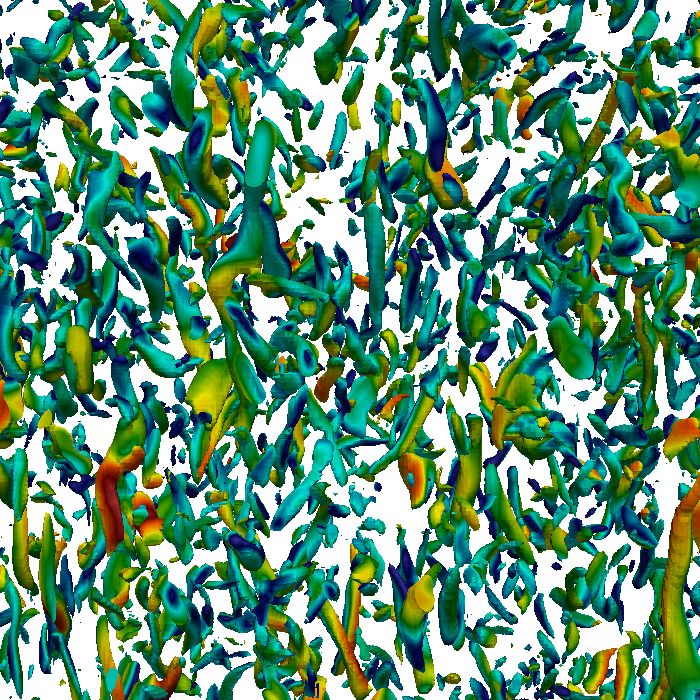
\includegraphics[width=0.95\linewidth]{./Abbildungen/256_velocity_4.png}
        \caption{???}
        \label{256_velocity}
    \end{minipage}%
    \begin{minipage}[t]{0.5\textwidth}
        \centering
        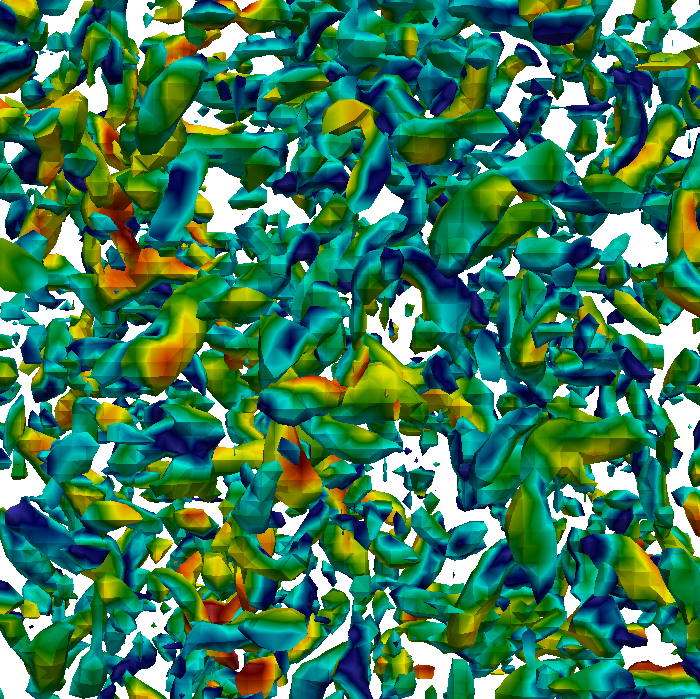
\includegraphics[width=0.95\linewidth]{./Abbildungen/64_velocity.png}
        \caption{??? Appendix A}
        \label{64_velocity}
    \end{minipage}
\end{figure}
Simulating only the larger-scale motions is called filtering, which means that the smaller-scale motions, also known as fluctuation, are filtered out. For further information on filter functions, the works of Pope \cite{turbulentFlows} should be considered. To model the filtered smaller-scale motions usually a subgrid-scale (SGS) model is used. According to Hickel (2007) the interference between explicit SGS and the truncation error can be exploited, i.e. the truncation error can serve as model of the effects of unresolved scales, which is therefore an implicit SGS model. Thus we call it implicit LES (ILES) \cite{implicitLES}. %als Zitat die Dissertation TUM Hickel
\subsection{Computational point particles}
\nomenclature[rmc]{$\lambda_\mathrm{c}$}{Ratio of physical point particles to computational point particles}
\nomenclature[rnp]{$N_\mathrm{p}$}{Number of physical point particles}
\nomenclature[rnc]{$N_\mathrm{c}$}{Number of computational point particles}
The high number of point particles requires even more computational resources for the particle-laden simulations than for the single-phase simulations. The main idea to reduce this requirement is to create clusters of point particles. For this purpose the ratio $\lambda_\mathrm{c}$ of physical point particles $N_\mathrm{p}$ to computational point particles $N_\mathrm{c}$ is introduced ($\lambda_\mathrm{c} = \frac{N_\mathrm{p}}{N_\mathrm{c}}$). To compensate this lack of particles, the coupling force is multiplied by $\lambda_\mathrm{c}$, due to the $\lambda_\mathrm{c}$-fold mass of the (cluster-)particles.
\pagebreak
\section{Results}
In this section the properties and results of the simulations that have been carried out will be presented. Special emphasis will be put on the turbulent kinetic energy budgets and their use to interpret the findings.
\subsection{Simulation properties \& assumptions}
In this section the results of the performed simulation will be pointed out with special emphasis on turbulent kinetic energy budgets and their influence on particle-laden turbulent flows.
\newline
All cases were simulated on a cubic domain and a cartesian grid using multiple grid refinement levels, $64^3$, $96^3$ and $128^3$ representing the LES hence the need to model smaller scales with SGS-models is present. Due to higher grid refinement in the $256^3$-case, these smaller scales can be directly simulated and therefore this simulation is a DNS.
\newline
The particle-free case was initialized using a seed-based random generator. At $t^* \approx 0.27$ a restart file is written out to initialize the subsequent simulation of the particle-laden isotropic turbulence. This file is then used to set up a second simulation including particle-load. Both these cases, DNSs of a single-phase and a particle-laden flow will used as reference for analyzing other results. Single-phase simulations will in the following be referred to as sP, and particle-laden ones as PP. The PP-simulation was set up to match the volume fraction $\phi_\mathrm{v}= 10^{-3}$ and mass fraction of $\phi_\mathrm{m}=1$. Both were constant in all simulations regarding particle clustering. The ratio of the densities for this set of simulations was set to $\frac{\rho_\mathrm{p}}{\rho} = 1000$, the particle diameter was set to match $d_\mathrm{p} \approx 0.6 \eta$. The injection of a million spherical point-particles was carried out interpolating the velocities of the surrounding fluid. At the timestep of injection the Stokes response time $\tau_\mathrm{ps}$ was 0.03497, the Prandtl number was 0.72 and $Re_\lambda$ was 57.9757. 
\subsection{The turbulent kinetic energy budget}
The change in kinetic energy of the fluid is in particle-laden decaying isotropic turbulence determined by the coupling rate $\Psi$, which describes the energy transfer between both fluid and particle phase, and the integral dissipation rate $\vec{\varepsilon}$:
\begin{equation}
\frac{\partial E_\mathrm{k}}{\partial t} = \Psi (t) - \vec{\varepsilon} (t).
\end{equation}
As mentioned before, the flow field is considered nearly incompressible, therefore the equation  for the viscous dissipation rate can be approximated by
\begin{equation}
 \epsilon (t) \approx 2 \mu \vec{\bar{S}}\vec{:}\vec{\bar{S}},
\end{equation}
were $\vec{:}$ denotes the inner tensor product. This rate can then be integrated over the full fluid domain $\Upsilon_\mathrm{f}$, leading to 
\begin{equation}
\varepsilon (t) = \int\limits_{\Upsilon_\mathrm{f}} \epsilon(t) \mathrm{d}V.
\end{equation}
As the dissipation rate is always of positive value, it acts a sink for the fluid's turbulent kinetic energy. In difference to that, the coupling rate can serve either as source or sink, depending on the acceleration of the particles \cite{mechanismsoftwowaycoupling}. The coupling rate for point-particles is defined as
\begin{equation}
\Psi (t) = \sum_{p=1}^{N_\mathrm{p}} \psi_\mathrm{p}= - \sum_{p=1}^{N_\mathrm{p}} \vec{F}_\mathrm{p} \times\vec{v}_\mathrm{p},
\end{equation}
describing the transfer of kinetic energy resulting from surface forces at each particle. 
\begin{equation}
\frac{\mathrm{d}E_\mathrm{kB}}{\mathrm{d}t} = - \Psi (t)
\end{equation}
therefore is the rate of change for global kinetic energy of the particles.
Additionally the particles change the fluid's rate of dissipation $\vec{\varepsilon}$ due to their volume forces. 
Schneiders et al. \cite{schneiders2017} therefore proposed a separation of dissipation rates for suspended heavy particles:
\begin{equation}
\frac{\partial E_\mathrm{k}}{\partial t} = \Psi (t) - \vec{\bar{\varepsilon}} (t) - \vec{\varepsilon}' (t).
\end{equation}
In this equation, $\vec{\bar{\varepsilon}} (t)$ displays the dissipation rate of the flow field and $\vec{\varepsilon}' (t)$ is the additional dissipation rate introduced by the injected point-particles. For $\rho_\mathrm{p} \gg \rho$ and the point-particle approach the equation
\begin{equation}
	\vec{\varepsilon}' = \sum_{p=1}^{N_\mathrm{p}} \vec{F}_\mathrm{p} \times (\vec{u}_\mathrm{p}-\vec{v}_\mathrm{p})
\end{equation}
can be formulated using the velocity of the fluid $\vec{u}_\mathrm{p}$ at the particle position.
\newline
\subsection{Simulation results}
\begin{figure}[h]
    \centering
    \begin{minipage}{0.5\textwidth}
        \centering
 	   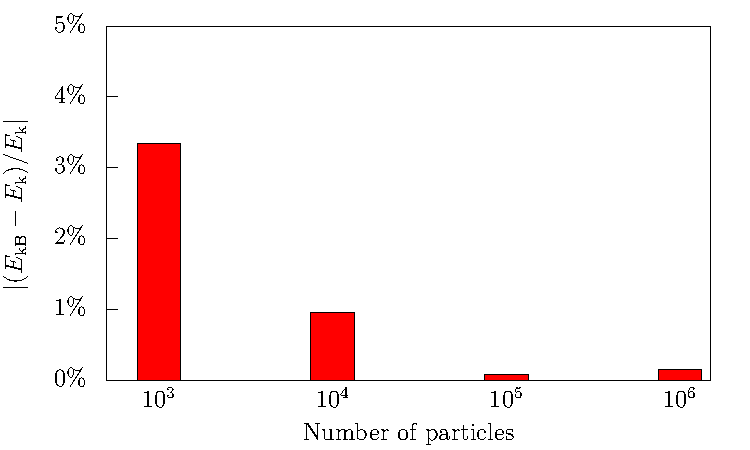
\includegraphics[width=\linewidth]{./Abbildungen/kineticEnergy_numberOfParticles.pdf}
    \end{minipage}%
        \begin{minipage}{0.5\textwidth}
        \centering
        \caption{Initializing different numbers of point-particles on a $128^3$-grid: An unsatisfactory inaccuracy can be observed for small numbers of particles}
	\label{kineticEnergy_numberofparticles}
    \end{minipage}
    \end{figure}
The first set of simulation was set up to investigate how different numbers of injected particles have an influence on the difference of turbulent kinetic energy of both particle and fluid. As mathematical description of turbulent flows is based on statistics, small numbers of particles can lead to questionable results. An example for the deviation in kinetic energy for different numbers of particles can be found in Fig. \ref{kineticEnergy_numberofparticles}. The normalized difference in kinetic energy $E_\mathrm{kB}$ of the particles and the flow itself $E_\mathrm{k}$ shows in this single simulation a correlation between particle number and accuracy in the simulation. Although this was just a single initialization of particles in a flow, it can be stated that simulations using only $10^3$ or even up to $10^4$ particles are not accurate enough for technical or scientific use of data. Simulations in other grid sizes show similar results.
\newline
\begin{figure}[h]
    \centering
    \begin{minipage}[t]{0.5\textwidth}
        \centering
 	   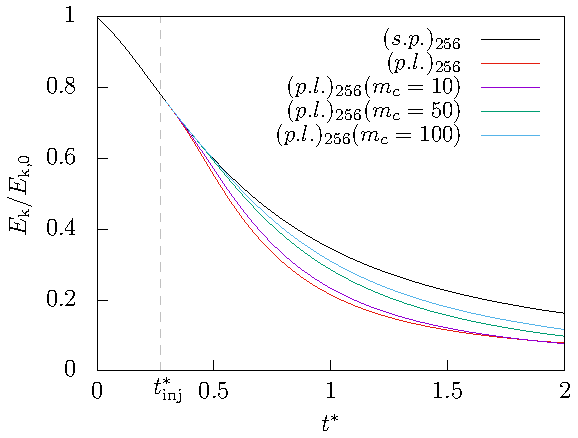
\includegraphics[width=\linewidth]{./Abbildungen/256/kineticEnergy_time.pdf}
	   \caption{Kinetic energy $E_\mathrm{k}$ normalized by its initial value $E_\mathrm{k,0}$ over time normalized by initial eddy turnover time. Shortly after the injection the PP-cases with separate from the sP-flow. The higher-clustered cases show less distinctions from the sP-case.}
	\label{kineticEnergy_time_256}
    \end{minipage}%
\begin{minipage}[t]{0.5\textwidth}
        \centering
        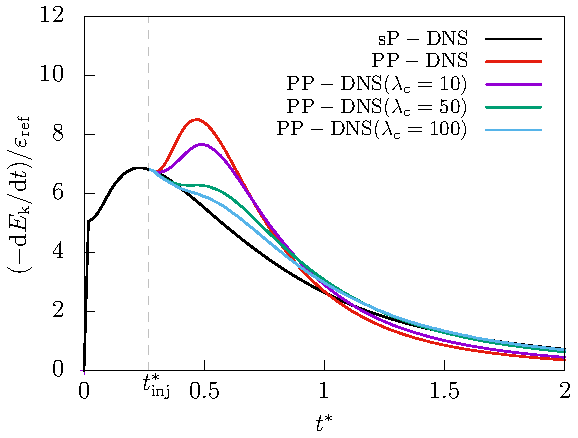
\includegraphics[width=\linewidth]{./Abbildungen/256/der(kineticEnergy)_time.pdf}
        \caption{Change in kinetic energy over time normalized by initial eddy turnover time. After $t^* \approx 1$ the unclustered PP-case shows a lower decay rate in kinetic energy than the sP-case.}
        \label{der_kineticEnergy_256}
    \end{minipage}
\end{figure}
\newline
The second set of simulations conducted in this work is set up to investigate the influence of particle clustering on the accuracy of the simulations with the goal to minimize computational effort, while still achieving high quality results. For this purpose, the variable $\lambda_\mathrm{c}$, which was established before, was implemented in the code. The simulations were then set up with the overall same number of a million particles, altering just $\lambda_\mathrm{c}$. It can be seen in Fig. \ref{kineticEnergy_time_256} and \ref{der_kineticEnergy_256} that the decay in kinetic energy from the injection point depends highly on the number of clustered particles. It can be stated that the flow's statistics for high $\lambda_\mathrm{c}$ converge approach the sP-case. 
\begin{figure}[h]
    \centering
    \begin{minipage}[t]{0.5\textwidth}
         \centering
        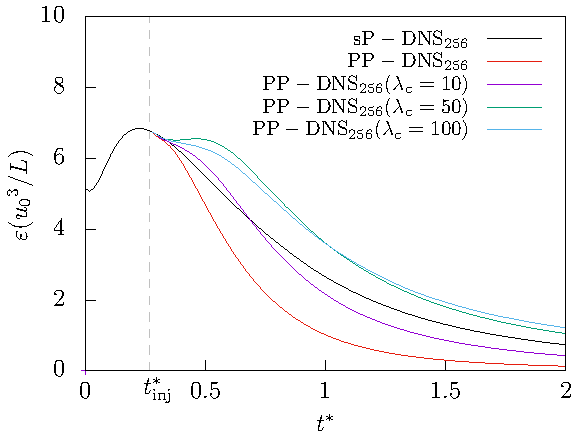
\includegraphics[width=\linewidth]{./Abbildungen/256/diss_time.pdf}
        \caption{Normalized dissipation rate $\vec{\varepsilon}$ over time normalized by initial eddy turnover time. The unclustered PP-case shows a lower dissipation rate than the sP-case. Highly clustered PP-cases show a higher dissipation rate.}
        \label{diss_time_256}
    \end{minipage}%
    \begin{minipage}[t]{0.5\textwidth}
        \centering
        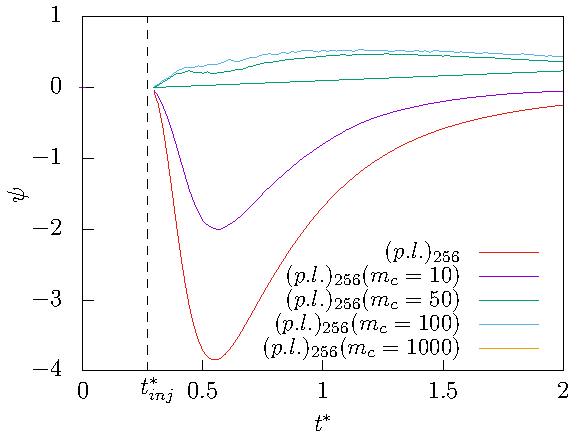
\includegraphics[width=\linewidth]{./Abbildungen/256/coupling_time.pdf}
        \caption{Normalized coupling rate $\Psi$ over time normalized by initial eddy turnover time. The PP-case without clustering show the lowest coupling rate. Both highly-clustered PP-cases show physically questionable behavior.}
        \label{coupling_time_256}
    \end{minipage}
\end{figure}
\newline
Fig. \ref{diss_time_256} and \ref{coupling_time_256} can be interpreted using the turbulent kinetic energy budget introduced earlier. The PP-case without clustering shows a lower dissipation rate than the sP-case, both highly-clustered cases show a higher rate over the monitored period of time. The coupling rate is negative all this time for the PP-cases with $\lambda_\mathrm{c}$ and positive for the higher-clustered cases. Both these effects form the change in kinetic energy in particle-laden isotropic flow found in Fig. \ref{der_kineticEnergy_256}.
\newline
Being very similar in the time shortly after the injection, the flow statistics diverge for different $\lambda_\mathrm{c}$ rapidly. The variables of these simulations one turnover time after the injection can be found in table \ref{table_values}. 
\begin{table}[h]
	\begin{center}
	\begin{tabular}{l l | c c c c c c }
	$\lambda_\mathrm{c}$& $\frac{m_\mathrm{c}}{m_\mathrm{V,cell}}$ & $\epsilon \frac{{u_0}^3}{L}$ & $\frac{\lambda}{L}$ & $\frac{\eta}{L} $ & $Re_\lambda$ \\
	\hline
	\hline
	1 &16.78 & 0.97& 0.039 & 0.0032 & 38.73 &\\
	10 &167.78 & 2.08 & 0.028 & 0.0026 & 28.66 &\\
	50 &838.86 & 3.51 & 0.024 & 0.0023 & 27.31 &\\
	100 &1677.72 & 3.51 & 0.025 & 0.0023 & 29.42 &\\
	\hline
	\end{tabular}
	\captionsetup{width=0.9\linewidth}
	\caption{Variables of the first set of simulations one turnover time after injection for the $256^3$-case}
	\label{table_values}
	\end{center}
	\end{table}
In Fig. \ref{particlekineticenergy_time_256} the kinetic energy of the particles is displayed. \textbf{Die Abbildungen passen inhaltlich nicht zueinander???}. Fig. \ref{vergleich_coupling_time_256} can be used to point out the difference between the results for LES and DNS. It is evident that a correlation between inaccuracy of the simulations and the refinement level of the grid exists. For the same relation of physical point particles to computational point particles the results show different behavior depending on the grids refinement level. The unclustered PP-case is included as reference. With $\lambda_\mathrm{c}=50$ being a relatively high ratio the $\mathrm{LES}_\mathrm{64}$ shows the most accurate results, the DNS shows the most inaccurate. This is due to the number of cells the force of the particles is projected on, which grows for each refinement step. It is therefore less critical to cluster particles in lower-resolution grids, although the results are not nearly as accurate as for the unclustered simulations. 
\newline
\begin{figure}[h]
    \centering
    \begin{minipage}[t]{.5\textwidth}
         \centering
        \includegraphics[width=\linewidth]{./Abbildungen/256/particlekineticenergy_time.pdf}
        \caption{Kinetic energy of the particles $E_\mathrm{kB}$ normalized by initial kinetic energy. The PP-case without clustering shows the biggest decay in kinetic energy. }
        \label{particlekineticenergy_time_256}
    \end{minipage}%
    \begin{minipage}[t]{0.5\textwidth}
        \centering
        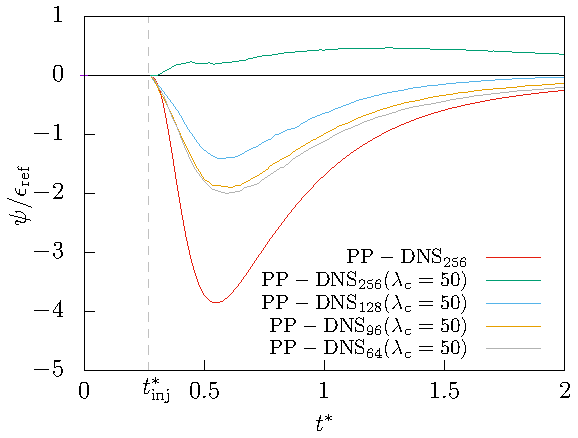
\includegraphics[width=\linewidth]{./Abbildungen/vergleich_coupling_time.pdf}
        \caption{Coupling Rate $\Psi$ with constant $\lambda_\mathrm{c}$ for various resolutions. A relation of resolution and accuracy can be observed.}
        \label{vergleich_coupling_time_256}
    \end{minipage}
\end{figure}
\newline
The computational savings of this method may be present, their effect is not as prevalent as it needs to be to compensate for the inaccurate results.
\pagebreak
\section{Conclusion and outlook}
In this work, two sets of simulations were carried out to evaluate a method for lowering computational effort. 
\newline
The results presented in this work show, that for a sufficiently exact simulation, particle clustering has to be treated with caution. Depending on the application maybe small numbers of clustered particles could be used, but the savings in computing time would not compensate the loss in accuracy. This is the case in particular high numbers of clustered particles at which the results get highly inaccurate. Maybe investigations on smaller numbers of clustered particles could follow, the space between 2 and 10 could be closed by simulations in the future to determine the real border for inaccurate results. 
\newline
Further investigation is needed regarding the second set of simulation, in which the goal was to find out which number of particles is necessary to get accurate results for the turbulent kinetic energy of the particles. The deviation of the averaged kinetic energy of the particles and the fluid should be zero. This difference converges to zero with high numbers of particles. The distribution of the experiment`s outcomes should match the well-known normal distribution, which leads to analyzing the standard deviation. Concluding, further simulations should be carried out until a sufficient standard deviation can be computed, from which an assumption about the accuracy of the initialization could be made.
\subsection*{Acknowledgements}
This work was supervised by Konstantin Fr\"ohlich, we would like to express our gratitude. Thank you for the chance of learning about turbulent flows and simulations, the advice and the deep insights in scientific work. We also appreciate the chance of writing this work at the Institute of Aerodynamics of the RWTH Aachen University.
\pagebreak
\section{References}
\nocite{*} %erm�glicht, dass auch Literatur, welche nicht zitiert wurde in der Bibliography auftaucht
\bibliography{Projektarbeit} %ruft die Bibliography-Datei auf
\bibliographystyle{plain} %setzt den Zitierstil
\pagebreak
\section{Appendix A}
\subsection*{Creating of pictures showing tubular structures}
The pictures used in the Introduction were generated using ParaView, an open-source-software developed by a joint-venture of Kitware and the Los Alamos National Laboratory. More information about the software can be found at www.paraview.org. To show the tubular structures in a turbulent flow, two filters were used: One was the AIALambda2Criterion1-Filter and the other one was the ISOVolume1-Filter. These filters were then set to visualize the velocity of the flow colored by magnitude. To diversify the different velocity-magnitudes, a rainbow-colorscheme was used. 
\end{document}
